\chapter{Modelos de consenso mejorados} \label{cap3}

En este capítulo se abordarán los primeros estudios sobre swarming realizados por Cucker Smale así como los modelos de consenso mejorados que toman como referencia principal y añaden un control heurístico que afecta a alguna de las variables, para potenciar el consenso.%el de los primeros centrándose en mejorar algunas de las variables para modificar el modelo


\section{Introducción}\label{s3_1}
La auto-organización de grupos en los que no existe un líder es un comportamiento común de ciertos animales que comúnmente se han llamado sociales como pueden ser algunos insectos, peces o aves. Como se ha podido ver en el capítulo \ref{cap2}, dar una explicación matemática a este comportamiento ha supuesto siempre un reto difícil de resolver debido a la alta complejidad que supone comprender el comportamiento individual y colectivo de dichos seres vivos resultando en un campo de estudio que hoy en día se divide en varias vertientes.

Muchos de estos modelos se basan en el comportamiento individual de cada uno de los componentes del grupo, proporcionando para cada uno de ellos una ecuación para explicar la evolución de la posición, velocidad u otras características. Estos modelos se llaman `Modelos basados en individuos' (IBMs por su traducción al inglés \textit{Individual-Based Models}). Las estrategias de estos modelos son muy variadas y pueden basar sus cálculos en premisas muy diferentes como puede ser ofrecer reglas para el movimiento de cada individuo para que sea lo más real posible, extraer las características básicas de estos modelos y tratar de comprender cuándo existe un comportamiento colectivo para poder profundizar mediante modelos más complejos, definir el comportamiento en función de unas condiciones iniciales, o buscar una alineación más rápida. 

Por tanto, conocer el comportamiento animal, proporciona retos y direcciones interesantes a seguir para la investigación matemática, y partir de modelos básicos que nos permitan conocer con mayor exactitud el comportamiento individual de los animales, nos da la oportunidad de seguir evolucionando hacia modelos más complejos que definan el comportamiento colectivo. En este capítulo se van a repasar tres modelos que se consideran básicos en la investigación del \textit{Swarming} y que han sido objeto principal de estudio en el presente trabajo.


\section{Cucker-Smale} \label{s3_2}
\subsection{Contexto} \label{s3_2_1}
Steve Smale es un matemático estadounidense doctorado por la Universidad de Michigan. Son conocidos sus contribuciones en Topografía y en Geometría diferencial. Recibió la Medalla Fields por demostrar el Teorema de Poincaré para dimensiones iguales o mayores que cinco \cite{StephenSmaleBio}. Son muchos sus reconocimientos, entre los que destacan también El Premio Veblen Prize para Geometría, de la Sociedad Matemática Americana en 1966 o la Medalla Nacional de Ciencia.

Juan Felipe Cucker Farkas es un matemático e informático uruaguayo y catedrático en la City University of Hong Kong. Es reconocido por ser especialista en Teoría de la Complejidad y por su relación con el condicionamiento de problemas numéricos. Durante su trayectoria profesional ha publicado numerosos artículos sobre las matemáticas de procesos emergentes junto con Steve Smale \cite{FelipeCuckerBio}.

El trabajo de ambos matemáticos sobre la emergencia en las formaciones de vuelo ha sido profusamente citado, hasta el punto de que en la actualidad se pueden encontrar en la literatura un buen número de artículos que toman este modelo (conocido como Cucker-Smale) como punto de partida de sus investigaciones.

\subsection{Modelo de Cucker-Smale} \label{s3_2_2}
Como se ha visto en el capítulo anterior, los animales sociales tienden a mostrar un comportamiento común en sus actividades, ya sea en la construcción de una colmena, en la recolección de comida, o en las migraciones. En cuanto a estas últimas se observó que bajo algunas condiciones iniciales, por ejemplo en sus posiciones y velocidades, el estado de la bandada converge a uno en el que todas las aves vuelan con la misma velocidad. Es por esto que gran parte del estudio que ocupa a Felipe Cucker y Steve Smale es la justificación matemática del consenso que tiene lugar cuando una bandada de pájaros se mueve. Si las premisas que se definen no se cumplen, entonces se produce la divergencia de las aves. Cabe mencionar que el modelo que proponen estos dos autores, tiene como punto de partida, el modelo analítico  de Vicsek \cite{vicsek1995novel}, del que se ha hablado anteriormente en el capitulo \ref{s2_2_2}, pero aportando un enfoque en el que la convergencia dependa únicamente de las condiciones del estado inicial.

El modelo Vicsek, se apoya en la idea de que un pájaro $i$ ajusta su velocidad en función de la velocidad media de la bandada a la que pertenece. Para poder profundizar en el modelo de Cucker Smale, se recuperan las ecuaciones vistas en el capítulo \ref{s2_2_4} para facilitar la lectura. Para aumentar la fidelidad del modelo de Vicsek a la realidad, Cucker y Smale postulan el siguiente comportamiento: cada ave ajusta su velocidad añadiéndole un promedio ponderado de las diferencias de su velocidad con las de las otras aves. Es decir, en un tiempo $t \in \mathbb N$  y para el pájaro $i$.

\begin{equation}\label{eq:CS1}
    v_{i}(t+1)-v_i(t)=\sum_{j=1}^{k} a_{ij}(v_{j}(t)-v_{i}(t))
\end{equation}

De esta manera se define mediante $a_{ij}$ la manera en la que las aves se influyen entre sí en función de la distancia, para lo cual es razonable asumir que sea inversamente proporcional a la distancia entre los pájaros y de esta manera los pájaros más cercanos tendrán mas peso que los más alejados. La forma matemática que asume esta variable según los autores es la siguiente función monótona no-creciente:

\begin{equation}\label{eq:CS2-aij}
    a_{ij} = a(||x_{i}-x_{j}||^2) = \frac{K}{(\sigma^2 +||x_{i}-x_{j}||^2)^\beta}
\end{equation}

\noindent donde $K,\sigma>0$ y $\beta>0$ son constantes que definen el comportamiento social del grupo. 

Una situación simplificada de un sistema de partículas particular puede definirse para $i = 1,...,N$ donde $\beta > 0$ es la constante que define la fuerza de influencia que tienen las aves en función de la distancia y $x_i \in \mathbb{R}^d, v_i \in \mathbb{R}^d$ son los parámetros que definen el estado y el consenso respectivamente. 

\begin{equation}\label{eq:CS5GeneralBeta} 
    \left\lbrace
    \begin{array}{ll}
        \dot{x}_{i}(t)=v_{i}(t) ,\\
        \dot{v}_{i}(t)= \displaystyle{\frac{1}{N}\sum_{j=1}^{N}\frac{v_{i}-v_{j}}{(\sigma^2+||x_{i}-x_{j}||^2)^\beta}}
    \end{array}
    \right.
\end{equation}

Este modelo representado por el sistema de ecuaciones \ref{eq:CS5GeneralBeta} propuesto por Cucker y Smale representa la \textit{capacidad de consenso} para un grupo de $N$ agentes capaces de interactuar entre sí bajo un mismo plano 2D. Aunque en un principio su estudio tenía como objetivo describir la formación y evolución de lenguajes \cite{cucker2007emergent}, debido a su simplicidad también se ha utilizado para relacionarlo con la capacidad de consenso de las bandadas de pájaros \cite{cucker2007mathematics}. 

El principal resultado de este modelo es su capacidad para definir el consenso del grupo en función del parámetro $\beta >0$. Definiendo una $\beta \leq 1/2$, se configura el sistema con en la cual los agentes guardan una interacción social de larga distancia bastante fuerte, garantizando la convergencia de la bandada a una velocidad común tanto para tiempo continuos como discretos.  Configurando una $\beta > 1/2$ dicha convergencia sólo está garantizada bajo unas condiciones concretas de posición y velocidades iniciales.


\subsubsection{Ejemplo 1: 2 agentes}\label{example1}
Para poder entender mejor este modelo, se puede utilizar un simple ejemplo en el que interactúan únicamente dos agentes. Se toma como referencia el sistema de ecuaciones \ref{eq:CS5GeneralBeta} y se establece que los 2 agentes se mueven en $\mathbb{R}$ con una posición y velocidad en un tiempo $t$, $(x_1(t),v_1(t)$ y $x_2(t),v_2(t)$. Por simplicidad, también se asume que $\beta=1, K=2$ y $\sigma=1$. El estado relativo del sistema viene dado por $x(t)=x_1(t)-x_2(t)$ y  el parámetro de consenso relativo por $v(t) = v_1(t) - v_2(t)$. Por tanto, el modelo \ref{eq:CS5GeneralBeta} se transforma en:


\begin{equation*}
    \left\lbrace
    \begin{array}{ll}
        \dot{x}=v ,\\
        \dot{v}= \displaystyle{-\frac{v}{1+x^2}}
    \end{array}
    \right.
\end{equation*}

\noindent con unas condiciones iniciales $x(0)=x_0$ y $v(0)=v_0>0$ e integrando $\dot{v}=-\dot{x}/(1+x^2)$, la solución de este sistema será:

\begin{equation*}
    v(t)-v_0=-\arctan x(t) + \arctan x_0
\end{equation*}


Si las condiciones iniciales satisfacen $|\arctan x_0 + v_0| < \pi/2$, entonces no se llegaría a un consenso en un tiempo finito y por tanto el estado relativo principal $|x(t)|$ está acotado uniformemente por $\tan(|\arctan x_0 +v_0|)$, de lo contrario carecería de velocidad.

A parte de los futuros estudios que surgen a raíz de éste y que se van a comentar en las siguientes secciones, existen una gran cantidad de modelos de Cucker-Smale aplicados de diferentes puntos de vista. Un estudio que emplea Cucker-Smale, es el realizado por Eitan Tadmor y Sebastien Motsch que en \cite{motsch2014heterophilious} explican su razón por la que se llega al consenso aplicado a la teoría de los grafos. Young-Pil Choi y Jan Haskovec en \cite{choi2016cucker} estudian el modelo de Cucker Smale con retardo de tiempo un aplican pesos diferentes de interacción entre cada uno de sus individuos para conseguir la convergencia del vector velocidad. Recientemente en la escuela de Ingeniería Industrial de Toledo se han realizado dos trabajos de interés que utilizan este modelo para aplicarlo a sus estudios y en los cuales por una parte se repasa una relación de modelos de Cucker Smale enfocados desde el punto de vista de la teoría de control aportando simulaciones \cite{jb2019tfg, ggl2019tfg} y por otra parte se propone un modelo físico para implementar en un sistema multiagente \cite{rc2019tfg, jg2020tfg}. Adicionalmente a estas referencias, existen numerosos artículos \cite{carrillo2010particle, albi2013binary, ha2008particle} que modifican el modelo de Cucker Smale, todos con el objetivo común de poder controlar en función de una serie de parámetros el movimiento de una agrupación de animales. 

%\begin{itemize}
%\item cono de visión \textcolor{red}{sin haber leido el enlace, ¿ES EL MISMO CONO DE VISIÓN AL QUR SE %HACE REFERENCIA EN AOKI \ref{s2_2_1}} \todo{revisar articulo %https://www-m15.ma.tum.de/foswiki/pub/M15/Allgemeines/OldNews/bookfinal.pdf} 
%\end{itemize}



\section{Modelos de Cucker-Smale mejorados}\label{s3_3}

\subsection{Modelo CCR} \label{s3_3_1}
En este artículo \cite{canizo2010collective},  J. A. Cañizo, J. A. Carrillo y J. Rosado explican algunos de los IBMs (\textit{Individual-Based Models}) aplicados al \textit{swarming} explicando de forma muy concisa algunos conceptos muy importantes de estos modelos como son la atracción, repulsión y orientación. Igualmente, dedican una parte para mostrar algunas pruebas sobre el comportamiento del modelo de Cucker-Smale y sus variantes. 

Cada individuo es influenciado de una manera diferente por otros individuos de su mismo grupo, en fucnión de su posición relativa, distinguiendo 3 zonas
\begin{figure}[h!]
    \centering
    {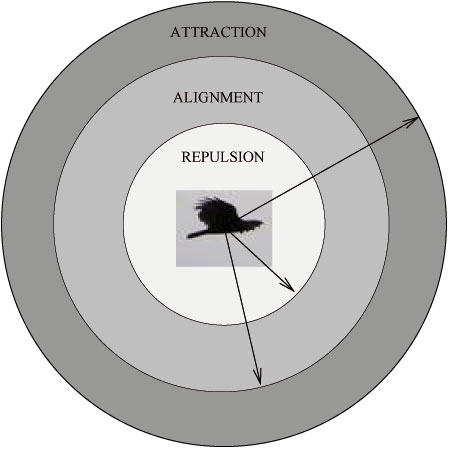
\includegraphics[height=6cm]{fig/cap03/3zones.png}}
    \caption{Modelo de las 3 zonas}
    \label{fig:3zonesModel}
\end{figure}

La zona interior es la llamada zona de repulsión o zona vital en la cual el individuo tiende a rechazar cualquier contacto con el que esté en esa zona, distanciándose. La zona de alineamiento o de orientación es en la cual tiende a igualar el mismo comportamiento que los individuos que están en esa zona. Por último, la zona de atracción o de socialización, es en la cual, los individuos que se encuentran en esa zona se acercan al individuo evitando estar lejos de los demás animales que están en esa región. Aunque el comportamiento de un grupo de animales se basa en rasgos generales en estas 3 zonas conceptuales, la realidad es que para poder reproducir un comportamiento de enjambre realista hay que incluir interacciones mucho más complicadas.

Por su parte, para demostrar que se consigue el consenso en el modelo general de Cucker Smale, los autores citados, proponen uno más general en el cual el promedio tiene en cuenta el módulo de la velocidad relativa ($ |v_{i}-v_{j}|^{p-2} $) de sus individuos (\ref{eq:CSArbor}). Obsérvese que para el valor $p = 2$ se obtiene el modelo inicial de Cucker-Smale. Mediante este modelo actualizado, demuestran que el consenso del grupo ocurre en un tiempo finito para 0 < p < 2 y 0 < $\beta$ <1/2 y con una velocidad algebraica si 2 < p < 3 - 2$\beta$ en contraste con la velocidad exponencial obtenida para el modelo estándar de Cucker-Smale con p = 2 y 0 < $\beta$ < 1/2


\begin{equation}\label{eq:CSArbor} 
    \left\lbrace
    \begin{array}{l}
        \dot{x}_{i}(t)=v_{i}(t) \\
        \dot{v}_{i}(t)= \displaystyle{\frac{1}{N}\sum_{j=1}^{N}a_{ij}(v_{j}-v_{i})|v_{i}-v_{j}|^{p-2}}
    \end{array}
    \right.
\end{equation}

Para concluir, en este artículo (\cite{canizo2010collective}) se propone un modelo en base al de atracción-repulsión (\ref{eq:attractionRepulsion}) y al general de Cucker-Smale (\ref{eq:CS5GeneralBeta}) al que llaman  ``modelo de las 3 zonas'':

\begin{equation}\label{eq:Arbor3zonesModel} 
    \left\lbrace
    \begin{array}{l}
        \dot{x}_{i}(t)=v_{i}(t) \\
        \dot{v}_{i}(t)=\displaystyle{-\frac{1}{N}\sum_{j\neq 1}\nabla U(|x_{i}-x_{j}|)+\frac{1}{N}\sum_{j=1}^{N}a_{ij}(v_{j}-v_{i})}
    \end{array}
    \begin{array}{r}
        (i = 1, ..., N) \\
        (i = 1, ..., N)
    \end{array}
    \right.
\end{equation}

En este modelo los individuos tienden a adoptar todos la misma velocidad, tal y como sucede en el modelo General de Cucker Smale, pero además consiguiendo que se agrupen todos los individuos.

\subsection{Modelo de Trelat} \label{s3_3_2}
Como se ha visto hasta ahora, el modelo de Cucker-Smale y sus diferentes mejoras, sólo llegan al consenso bajo ciertas condiciones iniciales, aunque los esfuerzos de todos los estudios se centran en obtener el modelo más óptimo para que esto ocurra. Existen muchas variaciones y extensiones del modelo de Cucker Smale, cada uno intentando resolver algunos de los problemas que puede tener ese modelo, teniendo en cuenta o añadiendo ciertos factores como aparición de ruido, fuerzas que eviten la colisión, tolerancia a errores, etc.

Para Trelat, una mayor optimización del modelo significará un menor gasto energético para que el consenso del grupo se consiga. La cita que mejor explica el razonamiento que utiliza en sus estudios es la siguiente: ``en vez de controlar a un mayor número de agentes con impulsos más pequeños, hay que actuar de manera más contundente sobre un menor número de líderes'' \cite{caponigro2015sparse}. Para entender mejor el modelo de Trelat, se debe entender antes cómo controlar el modelo de Cucker Smale. Cuando el consenso de un grupo no se ha conseguido mediante la autoorganización del grupo como puede verse en el \ref{example1} en el caso de $|arctan(x_0) + v_0| > \pi/2$ es natural
preguntarse si es posible provocar que el grupo consiga el consenso mediante una fuerza o acción externa. 

\begin{equation}\label{eq:trelat_CS}
    \left\lbrace
    \begin{array}{ll}
        \dot{x}_{i}(t)=v_{i}(t) \\
        \dot{v}_{i}(t)= \displaystyle{\frac{1}{N}\sum_{j=1}^{N} a(||x_i(t)-x_j(t)||)(v_{j}(t)-v_{i}(t))}
    \end{array}
    \right.
\end{equation}

Los autores de este estudio se refieren a este tipo de consenso con el término ``organización mediante intervención''. Para esta intervención, matemáticamente se añade al sistema propuesto por Cucker Smale \ref{eq:trelat_CS} la variable de control $u_i$. Con este término, Trelat lo que consigue es que el individuo $i$ se mueva hacia una dirección común, aportándole un empujón extra a cada individuo del grupo. 

\begin{equation}\label{eq:CSTrelat_control}
    \left\lbrace
    \begin{array}{l}
        \dot{x}_{i}(t)=v_{i}(t) \\
        \dot{v}_{i}(t)= \displaystyle{\frac{1}{N}\sum_{j=1}^{N}a(||x_{j}(t)-x_{i}(t)||)(v_{j}(t)-v_{i}(t))+u_{i}(t)}
    \end{array}
    \right.
\end{equation}

En esta ocasión, la variable de control $u_i$ se selecciona en base a la perpendicular del vector, proporcionando un ``empujón'' perpendicular al individuo en base a la siguiente ecuación. 

\begin{equation}\label{eq:Trelat_ui}
    u_i(t) = 
    \left\lbrace
    \begin{array}{l}
        \displaystyle{-\alpha_i \frac{v_{\perp_{i}}(t)}{||v_{\perp_{i}}(t)||}} \\
        0
    \end{array}
    \right.
\end{equation}

\noindent en la cual $\alpha_j$ es una constante que por simplificar, se iguala a 1, $v_{\perp_{i}}(t)$ del numerador es el vector perpendicular que va a modificar la dirección actual del individuo, y $||v_{\perp_{i}}(t)||$ en el denominador es la dirección en la que se va a proporcionar el cambio. 

Por tanto, en este estudio, lo que demuestran los autores es que en un tiempo finito el sistema consigue reunir las condiciones que Cucker y Smale dicen que asegura la convergencia a pesar de empezar en un estado que sin ningún tipo de control, el modelo inicial, no llegaría al consenso.
